\chapter{\label{cha: Graph Transformation}Model to Model Transformation}

\section{Introduction}
In this chapter, we define the modelisation Levels, and the model-to-model transformation, specifically the graph transformation type, and ending with an overview about the AToM3 tool.

\section{Levels of Modilisation}

What do we mean when we use the word model. It has Several definitions among

\begin{enumerate}
\item A model is an abstraction of a system (real or language-based) allowing
To draw predictions or conclusions\cite{ch3-matters}. 
\item The central idea of modeling is to produce a reduced version of the system To determine and evaluate its salient properties\cite{ch3-selic}. 

\item A model is a simplification of a system designed with a purpose in mind.
The model should be able to answer questions in the current system. The responses provided by the model should be the same as those proposed by the system itself, provided that the questions are within the defined domain by the general objective of the system\cite{ch3-def}.

\end{enumerate}

meta-model is a model of a modeling language. The term "meta" means above.

A meta-model a language of Modeling at a higher level of abstraction than the modeling language itself\cite{ch3-applied}.


Meta-Modelling, which is the process of modelling formalisms. 
Formalisms are described as models described in meta-formalisms. 
The latter are nothing but expressive enough formalisms, such as Entity Relationship diagrams (ER) or UML class diagrams.

A model of a meta-formalism is called a meta-meta-model, a model of a formalism is called a meta-model\cite{ch3-meta2}.

Meta-model architecture allows a meta-model to be seen as a model, it is
Itself described by another meta-model. This allows all meta-models to be
Described by a single meta-model. This unique meta-model, known as a
Meta-model, is the key to meta-modeling because it allows all languages
Modeling to be described in a unified manner.


\subsection{Architercteur of Meta-Modeling}
The traditional meta-model architecture proposed by OMG is based on 4 Levels
described in this Figure \ref{fig:Pyramid of Meta-Level} \cite{ch3-doc, ch3-mml} .

\begin{enumerate}
\item \textbf{Model} is a simplified abstraction of a studied system, constructed in a
Particular intent. 

It should be able to be used to answer questions about the system

A system is a theoretical construct formed by the mind on a subject
Example, an idea that is implemented to explain a physical phenomenon that can
be represented by a mathematical model) 

\item \textbf{Meta Model} is a language that expresses models. It defines
Concepts as well as the relations between concepts necessary for the expression of models. 
A model is a possible construction of the metamodel in which it is defined.

In the Literature, a model is said to conform to the metamodel in which it is defined

\item \textbf{Meta Meta Model} is a language used to express metamodels. 
For Ability to interpret a meta-model requires a description of the language in which
It is written: a meta-model for meta-models. 
It is, of course, Meta-model by the term meta-meta-model. 

To limit the Number of levels of abstraction, the meta-meta-model 
must have the ability to describe itself, even. 
 

\end{enumerate}

MOF : (Meta-Object Facility) is set of Interfaces allow to define 
the syntax and semantic of modilisation language, is devloped by OMG\cite{ch3-doc, ch3-doc}.

\begin{figure}[th]
	\centering
		\includegraphics[0.5]{ch3/img/Pyramid}
	\caption{\label{fig:Pyramid of Meta-Level}Pyramid of Meta-Level\cite{ch3-doc}}
\end{figure} 

\pagebreak

\section{Model Transformation}
Transformation is a fundamental theme in computer science and software engineering. After all, computation can be viewed as data transformation. Computing with basic data such as numeric values
and with data structures such as lists and trees is at the heart of programming. Type systems in programming languages help ensure that operations are applied compatibly to the data \cite{ch3model}. 


\subsection{Transformation Categories}
In general, we can view transforming models to code as a special case of model-to- model transformations; we only need to provide a metamodel for the target programming language. However, for practical reasons of reusing existing compiler technology, code is often generated simply as text, which is then fed into a compiler. For this reason, we distinguish between model-to-code transformation (which would be better described as model-to-text since non-code artifacts such as XML may be generated) and model-to-model transformation. Several tools offer both model-to-model and model-to-code transformations \cite{ch3catego}.

\subsubsection{Model To Code}
In the model-to-code category, it is very basic code generation approach consists mechanism to traverse the internal representation of model and write code to a text stream, we distinguish between visitor-based and template-based approaches \cite{ch3catego}.
\subsubsection{Model To Model}
Model-to-model transformations translate between source and target models, which can be instances of the same or different metamodels, Most existing MDA tools provide only model-to-code transformations, we distinguish among direct-manipulation approaches, relational approaches, graph-transformation-based approaches \cite{ch3catego}.

\subsection{Transformation Languages and Tools}

\subsubsection{ATL :}
Transformation Language (Jouault et al., 2006) is a model transformation language and
toolkit developed and maintained by OBEO and INRIA-AtlanMod (Czarnecki and Helsen, 2006)\cite{ch3lang}.

\subsubsection{JTL :}
Janus Transformation Language (JTL) is a bidirectional model transformation language specifically designed to support non-bijective transformations and change propagation (Cicchetti et al., 2011)\cite{ch3lang}.

\subsubsection{ETL :}
Epsilon family (Kolovos et al., 2006) is a model management platform that provides transformation languages for model-to-model, model-to-text, update-in-place, migration and model merging transformations\cite{ch3lang}.

\subsubsection{Kermeta :} 
The Kermeta language was initiated by Franck Fleurey in 2005 , The Kermeta language borrows concepts from languages such as MOF, OCL and QVT\cite{ch3lang}.

\subsubsection{QVT :} 
The OMG has defined a standard for expressing M2M transformations, called MOF/QVT or in short QVT (Eclipse, 2008). Eclipse has two extension for QVT called QVTd (Declarative) and QVTo (Operational/Procedural)\cite{ch3lang}.

\subsubsection{MOFScript :} 
The MOFScript includes tools and frameworks for supporting model to text transformations, e.g., to support generation of implementation code or documentation from models\cite{ch3lang}.

\pagebreak


\section{Concept of Graph Transformation} 
The process of graph transformation consists in the iterative application of
Rule to a graph. Each rule application replaces a part of the graph, As defined in the rule. 
The mechanics of the graph transformation works as follows : 

\vspace{1cm}
\begin{algorithm}
\SetAlgoLined

\KwData{G : Graph Source , GG : Graph Grammar , R : one rule from GG , subG : sub
Graph from G , i : integer represent the priority of Rule ;
 i=0;}
\KwResult{G graph contain the graph target }

 \While{( \textbf{R} = ChooseFrom(\textbf{GG},i) ) != null}{
 	\While{( (\textbf{subG} = selectFrom(\textbf{G})) != null}{
 		\eIf{ not \textbf{subG}.isDoneWith(\textbf{R}) }{
			\textbf{R}.ApplyOn(\textbf{subG}) \linebreak
			\textbf{subG}.markAsDoneWith(\textbf{R})\linebreak
			print "We Applied Rule R on the subGraph subG" 
		}{
			print "This rule is applied before that on the same sub graph" 
		}
 	}
 	\textbf{i} = \textbf{i} + 1 \;
}
 
 \caption{application of graph transformation}
\end{algorithm}

\vspace{0.5cm}
 
This operation is based on set of rules respecting a particular 
syntax, called the grammar model of Graph.
Before starting apply rules we execute initial action, 
its prepare the envirenement to apply these rules
and ending with Final Action, it about cleaning the after these rules\cite{ch3-bid, ch3-spec}.


\vspace{0.5cm}
\begin{figure}[th]
	\centering
		\includegraphics[scale=0.52]{ch3/img/transGrammar}
	\caption{\label{fig:Cycle of Tranformation}Cycle of Transformation\cite{ch3-img}}
\end{figure} 

\pagebreak
\section{Graph Grammar} 
Every Graph Grammer contain a set of rules to use in graph transformation
and it is define by\cite{ch3-doc, ch3-spec} :
R = (LHS, RHS, K, glue, emb, cond). 
\begin{itemize}
\newcommand{\localtextbulletone}{\textcolor{gray}{\raisebox{.45ex}{\rule{.6ex}{.6ex}}}}
\renewcommand{\labelitemi}{\localtextbulletone}
\item LHS graph of left part.
\item RHS graph of right part.
\item A subgraph K of LHS.
\item A glue occurrence of K in RHS that connects the subgraph with the part graph right.
\item An embedding relation emb which connects the vertices of the graph on the left-hand side
And those of the graph on the right-hand side.
\item A set cond which indicates the conditions of application of the rule
\end{itemize}

Applying a rule R = (LHS, RHS, K, glue, emb, cond) to a graph G produced in
Result a graph H according to the following five steps

\begin{figure}[th]
	\centering
		\includegraphics[scale=0.9]{ch3/img/rules}
	\caption{\label{fig:Rule Application}Rule Application\cite{ch3-img}}
\end{figure} 

\begin{enumerate}
\item Choose an instance of the left-hand LHS graph in G.
\item Check the conditions of application according to Cond.
\item Remove the occurrence of LHS (up to K) from G and the hanging arcs (all
Arcs having lost their sources and / or their destinations). This provides the graph of
Context D of LHS which left an occurrence of K
\item
Paste the context graph D and the RHS right-hand graph according to the occurrence
Of K in k = 1, .., $\infty$ D and in RHS, it is the construction of the union of disjunction
Of D and RHS, and for each point in K, identify the corresponding point in
D with the corresponding point in RHS
\item
Press the right-hand graph in the LHS context graph following the
Embedding relation emb: for each incident arc removed with a vertex v in
D and with a vertex v1 in the occurrence of LHS in G, and for each vertex
V2 in RHS, a new incident arc is established (same label) with the image of v
And the vertex v2 provided that (v1, v2 ) belongs to emb. 
\end{enumerate}


 
\section{Transformation system} 

We define a graph transformation system as a rewriting system
Of graph that applies the rules of the graph grammar on its initial graph of
Iteratively by the Engine, until no more rules are applicable\cite{ch3-doc2, ch3-doc}.

\begin{enumerate}
\item Define the source and target Meta-Model 
\item Create the the source model according to the source Meta-Model 
\item Define transformation rules to Transform from source model into target model 
\end{enumerate} 
Finally the engine read source model and apply the transformation rules and write target model as the following Figure \ref{fig:Transformation System}
 
\begin{figure}[th]
	\centering
		\includegraphics[scale=0.4]{ch3/img/systemTran}
	\caption{\label{fig:Transformation System}Transformation System\cite{ch3-img}}
\end{figure} 

\section{AToM3}

AToM3 (A Tool for Multi-formalism and Meta-Modeling) is a tool for model-
Multi-paradigm model developed in the MSDL (Modeling, Simulation and
Design Lab) of the Computer Science Institute at McGill University Montreal, Canada\cite{Siteatom, ch3-atom3}.

It is Developed with the Python language in collaboration with Professor Juan de Lara de
The Autonomous University of Madrid (UAM), Spain 
AToM3 is developed to satisfy two main features that are 
\begin{enumerate}
	\item Meta-modeling 
\item The transformation of models
\end{enumerate}

The formalisms and models in AToM3 are described graphically. 
From a Meta-specification (example: in the Entity-relation formalism) of a formalism, AToM3
Generates a tool to visually manipulate (create and modify) the models described in
The specified formalism.

 The transformations of the models are realized by the rewriting
Graphs, which can be expressed in a declarative way as a model of
Grammar of graphs\cite{ch3-meta2}.

 figure \ref{fig:AToM3 Window} illustrates the interface of AToM3 

\begin{figure}[th]
	\centering
		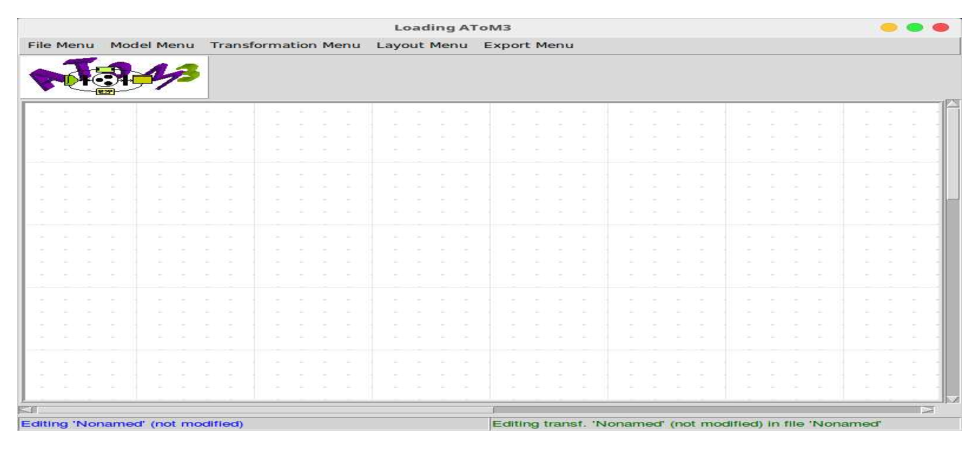
\includegraphics[scale=0.33]{ch3/img/atom3}
	\caption{\label{fig:AToM3 Window}AToM3 Window}
\end{figure} 
\vspace{1cm}
\subsection{Classes in AToM3}
In this work we use ClassDiagramm Formalism to create our Formalism 
or Meta-Model is built in the tool so we can load it and use it\cite{ch3-meta2}.
In AToM3 the meta-models can be constructed from Classes and
Relationships.

The description of classes and association relations consists of

\begin{minipage}{0.5\textwidth}
\begin{itemize}
\newcommand{\localtextbulletone}{\textcolor{gray}{\raisebox{.45ex}{\rule{.6ex}{.6ex}}}}
\renewcommand{\labelitemi}{\localtextbulletone}
\item Name
\item Attributes
\item Constraints
\item Action
\item Cardinalities
\item Appearance
\end{itemize}
\end{minipage} \hfill
\begin{minipage}{0.45\textwidth}
\begin{figure}[H]
\centering
		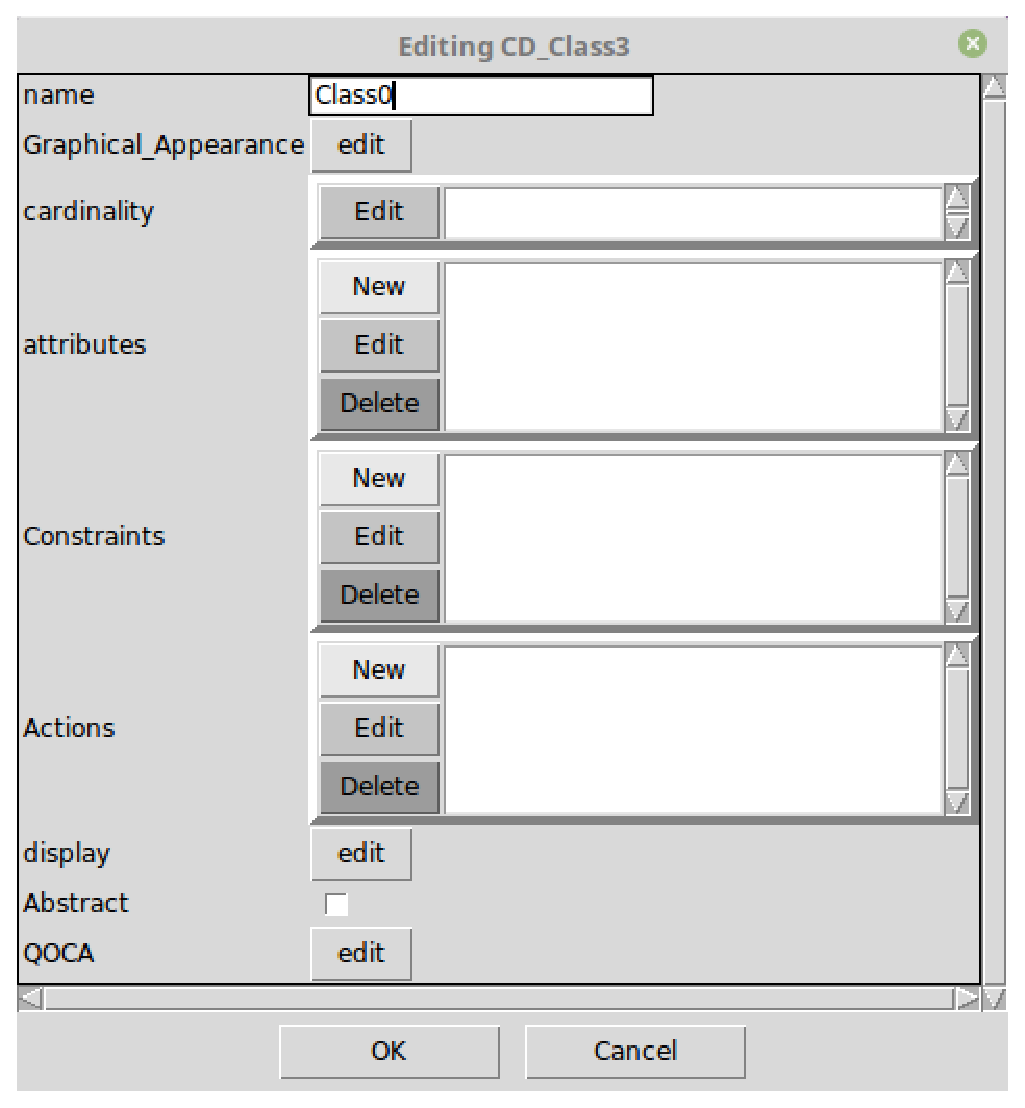
\includegraphics[scale=0.4]{ch3/img/class}
	\caption{\label{fig:Class Editor}Class Editor}
\end{figure}
\end{minipage}

\vspace{1cm}

\subsubsection{Constraint}

Constraints can be specified as OCL (Constraint Object Language) or Python
They have the following properties: 
\begin{itemize}
\newcommand{\localtextbulletone}{\textcolor{gray}{\raisebox{.45ex}{\rule{.6ex}{.6ex}}}}
\renewcommand{\labelitemi}{\localtextbulletone}
\item constraint name
\item triggering event like Drag, Move, Select ..
and launch this event before (pre-condition) or after (post-condition)
 
\end{itemize}
 

\begin{figure}[th]
	\centering
	\includegraphics[scale=0.37]{ch3/img/const}
	\caption{\label{fig:Constraint Editor}Constraint Editor}
\end{figure} 

\subsubsection{Action}

An action is similar to a constraint except that it has other effects and is a
Code in Pyton only, its have the same windows \ref{fig:Constraint Editor} 

They have the following properties :
\begin{itemize}
\newcommand{\localtextbulletone}{\textcolor{gray}{\raisebox{.45ex}{\rule{.6ex}{.6ex}}}}
\renewcommand{\labelitemi}{\localtextbulletone}
\item action name
\item triggering event: It can be either
	\begin{enumerate}
	\item Semantics such as saving a model
	\item Graphic or structural, such as moving or selecting an entity.
	\end{enumerate}
	
\item The execution is either
	\begin{enumerate}
	\item Before the event (precondition)
	\item After (pots-condition) 
	\end{enumerate}

\end{itemize}
 


\subsection{Graph Grammer in AToM3}
In AToM3, grammar is characterized by

\begin{minipage}{0.5\textwidth}

\begin{itemize}
\newcommand{\localtextbulletone}{\textcolor{gray}{\raisebox{.45ex}{\rule{.6ex}{.6ex}}}}
\renewcommand{\labelitemi}{\localtextbulletone}
\item An initial action.
\item A final action.
\item The set of rules. 
\end{itemize}

\end{minipage} \hfill
\begin{minipage}{0.45\textwidth}
\begin{figure}[H]
	\centering 
	\includegraphics[scale=0.5]{ch3/img/GraphGrammar}
	\caption{\label{fig:Graph Grammar Window}Graph Grammar Window}
\end{figure}
\end{minipage} 
\linebreak

Each rule consists of: 
A specific name for the rule, and priority indicator the order in which the rule is applied, and LHS \footnote{LHS:Left Hand Side}:which is a graph, RHS\footnote{RHS:Right Hand Side}:that can be a graph and the condition that must be checked before the rule is Applied, finally An action (a Pyton code) that must be executed after the rule is
Applied

\begin{figure}[th]
	\centering
 	\includegraphics[scale=0.38]{ch3/img/ruleEditor}
	\caption{\label{fig:Rule Editor}Rule Editor}
\end{figure} 

\section{Conclusion}
in this portion of our document, we represented the different type of transformation approach and we use the graph transformation approach, then we mentioned the tool AToM3.